\documentclass[a4paper, 12pt]{book}
% preamble.tex

\usepackage[utf8]{inputenc}
\usepackage[T1]{fontenc}
\usepackage[english]{babel} % Ho cambiato in italian, supponendo che la maggior parte del testo sia in italiano
\usepackage{amsmath}
\usepackage{amssymb}
\usepackage{graphicx}
\usepackage{hyperref}
\usepackage{geometry}
\usepackage{fontspec} % Utile per Xetex/LuaLaTeX ma mantenuto
\usepackage{booktabs}
\usepackage{amsthm}
\usepackage{enumitem}
\usepackage{caption}
\usepackage{thmtools}
\usepackage{standalone} % Già presente nel tuo elenco
\usepackage{tkz-euclide}
\usepackage{graphicx}
\usepackage[T1]{fontenc}
\usepackage{wesa}

% --- PACCHETTI AGGIUNTI PER LA FORMATTAZIONE ---
\usepackage{parskip}  % Aggiunge spazio tra i paragrafi (stile "blocco")
\usepackage{fancyhdr} % Per intestazioni e piè di pagina personalizzati

% --- IMPOSTAZIONI GEOMETRIA E FONT ---
\geometry{a4paper, margin=1in}

% Configura lo stile 'plain' (usato da \maketitle e \tableofcontents)
% per essere coerente con il piè di pagina
\fancypagestyle{plain}{
    \fancyhf{} % Pulisce
    \cfoot{\thepage} % Mette solo il numero di pagina
    \renewcommand{\headrulewidth}{0pt} % Niente linea su queste pagine
}

% Configurazione Header/Footer per le altre pagine
\pagestyle{fancy}
\fancyhead{} % Pulisce l'intestazione
\fancyfoot{} % Pulisce il piè di pagina
\fancyhead[L]{\nouppercase{\rightmark}} % Nome Sezione a sinistra (o Chapter)
\fancyhead[R]{\nouppercase{\leftmark}}  % Nome Capitolo a destra (o Sezione)
\fancyfoot[C]{\thepage} % Numero di pagina al centro
\renewcommand{\headrulewidth}{0.4pt}
\renewcommand{\footrulewidth}{0pt}


% --- DEFINIZIONI TEOREMI ---
% (Questa parte è cruciale per la tua struttura)
\newtheoremstyle{mythmstyle}%
    {}%
    {}%
    {\itshape}%
    {}%
    {\bfseries}%
    {}%
    { }%
    {\thmname{#1}\thmnumber{ #2}%
    \thmnote{: #3\addcontentsline{toc}{subsubsection}{{\itshape#1}: #3}}. }

% 2. Imposta questo stile come quello ATTUALE
\theoremstyle{mythmstyle}

\newtheorem{theorem}{Th}[section]
\newtheorem{definition}{Def}[section]
\newtheorem{proposition}{Prop}[section]
\newtheorem{corollary}{Cor}[section]
\newtheorem{algorithm}{Alg}[section]
\newtheorem{lemma}{Lemma}[section]
\newtheorem*{remark}{Rem}

% Definizioni utili per il Main file
\newcommand{\inputlesson}[1]{\clearpage\input{#1}\clearpage} % Comando per input lezione
\usepackage[x11names]{xcolor}
\usepackage{tikz}
\usepackage{amsmath} % Required for align environment
\usepackage{caption} % Required for \captionof outside float environments

\begin{document}
\setcounter{chapter}{1}
\setcounter{section}{0}
\chapter*{Appendix A: Transforms}
\addcontentsline{toc}{chapter}{Appendix A: Transforms}

\begin{purplebox}[DigiCom/Notes]
This appendix reviews several Fourier transforms, instrumental in the transition between the time and the frequency domains, as well as the Z-transform.
\end{purplebox}

% Hand-drawn graph reproduction (Square Wave)
\begin{center}
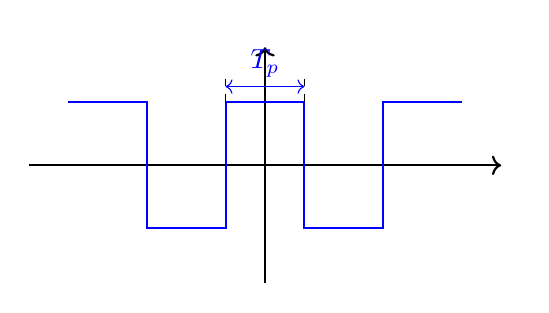
\begin{tikzpicture}
    % Axes
    \draw[->, thick] (-3,0) -- (3,0) node[right] {};
    \draw[->, thick] (0,-1.5) -- (0,1.5) node[above] {};
    
    % Square Wave (blue)
    \draw[blue, thick] (-2.5,0.8) -- (-1.5,0.8) -- (-1.5,-0.8) -- (-0.5,-0.8) -- (-0.5,0.8) -- (0.5,0.8) -- (0.5,-0.8) -- (1.5,-0.8) -- (1.5,0.8) -- (2.5,0.8);
    
    % Labels
    \draw[blue, <->] (-0.5, 1.0) -- (0.5, 1.0) node[midway, above] {$T_p$};
    \draw[dashed] (-0.5, 0.8) -- (-0.5, 1.1);
    \draw[dashed] (0.5, 0.8) -- (0.5, 1.1);
\end{tikzpicture}
\end{center}

\section{Fourier transforms}

\subsection{Continuous-time Fourier transform}

A well-behaved continuous-time function $x(t)$ and its Fourier transform $x(f)$ are related by the analysis and synthesis equations

\begin{align}
    \text{Analysis} \quad & x(f) = \int_{-\infty}^{\infty}x(t)e^{-j2\pi ft}dt \tag{A.1} \\
    \text{Synthesis} \quad & x(t) = \int_{-\infty}^{\infty}x(f)e^{j2\pi ft}df. \tag{A.2}
\end{align}

A detailed account of the technical conditions that are necessary for a Fourier transform to exist is beyond the scope of this book, and interested readers are referred for instance to [1053]. It suffices to say that all physically realizable signals do have Fourier transforms. For our purposes, therefore, we can take "well-behaved" to simply mean a signal for which the integral in (A.1) exists.

Those properties of the continuous-time Fourier transform that are invoked somewhere in the text are listed in Table A.1. Likewise, relevant Fourier transform pairs are presented in Table A.2.

\subsection{Continuous-time Fourier series}

Periodic functions do not fall under the umbrella of well-behaved functions and yet they are very important in the analysis of communication signals. This obstacle can be side-stepped through the definition of the Fourier series and by invoking the Dirac delta function, $\delta(\cdot)$.

Consider a periodic signal $x(t)$ whose period, $T>0$, is the smallest real number such that $x(t)=x(t+T)$. The continuous-time Fourier series of such signal is defined as

\begin{align}
    \text{Analysis} \quad & x[n]=\frac{1}{T}\int_{0}^{T}x(t)e^{-j\frac{2\pi}{T}nt}dt \tag{A.3} \\
    \text{Synthesis} \quad & x(t)=\sum_{n}x[n]e^{j\frac{2\pi}{T}nt}. \tag{A.4}
\end{align}

\begin{yellowbox}[REMEMBER ALL OF THAT]
\begin{center}
\captionof{table}{Continuous-time Fourier transform properties}
\small
\begin{tabular}{@{}lll@{}}
\toprule
\textbf{Property} & \textbf{Aperiodic signal} $x(t)$ & \textbf{Fourier transform} $x(f)$ \\ \midrule
Linearity & $ax(t)+b~y(t)$ & $ax(f)+by(f)$ \\
Time shift & $x(t-t_{0})$ & $e^{-j2\pi ft_{0}}x(f)$ \\
Conjugation & $x^{*}(t)$ & $x^{*}(-f)$ \\
Time reversal & $x(-t)$ & $x(-f)$ \\
Time scaling & $x(at)$ & $\frac{1}{|a|}x(\frac{f}{a})$ \\
Convolution & $x(t)*y(t)=\int x(\tau)y(t-\tau)d\tau$ & $x(f)y(f)$ (CONV into PRODUCTS) \\
Autocorrelation & $x(t)*x^{*}(-t)$ & $|x(f)|^{2}$ \\
Modulation & $x(t)e^{j2\pi f_0 t}$ & $x(f-f_{0})$ \\
Conjugate symmetry & $x(t)$ is real & $x(f)=x^{*}(-f)$ \\
Duality & $x(t) \leftrightarrow x(f)$ & $X(t) \leftrightarrow x(-f)$ \\
Parseval's theorem & $\int x(t)y^{*}(t)dt = \int x(f)y^{*}(f)df$ & $\int |x(t)|^{2} dt = \int |x(f)|^{2} df$ \\ \bottomrule
\end{tabular}
\end{center}
\end{yellowbox}

\begin{table}[h]
\centering
\caption{Continuous-time Fourier transform pairs}
\begin{tabular}{@{}ll@{}}
\toprule
\textbf{Time-domain} & \textbf{Frequency-domain} \\ \midrule
Impulse $\delta(t)$ & 1 \\
Constant function 1 & $\delta(f)$ \\
Complex exponential $e^{j2\pi f_{0}t}$ & $\delta(f-f_{0})$ \\
Cosine $cos(2\pi f_{0}t+\theta)$ & $\frac{1}{2}[e^{j\theta}\delta(f-f_{0})+e^{-j\theta}\delta(f+f_{0})]$ \\
Sine $sin(2\pi f_{0}t+\theta)$ & $\frac{1}{2j}[e^{j\theta}\delta(f-f_{0})-e^{-j\theta}\delta(f+f_{0})]$ \\
Impulse train $\sum_{k}\delta(t-kT)$ & $\frac{1}{T}\sum_{n}\delta(f-\frac{n}{T})$ \\
Rectangular pulse $rect(\frac{t}{T})=\begin{cases}1&|t|\le\frac{T}{2}\\ 0&else\end{cases}$ & $T~sinc(fT)=\frac{sin(\pi fT)}{\pi f}$ \\
Sinc pulse $sinc(Wt)=\frac{sin(\pi Wt)}{\pi Wt}$ & $\frac{1}{W}rect(\frac{f}{W})$ \\ \bottomrule
\end{tabular}
\end{table}

The continuous-time Fourier series creates as an output a weighting of the fundamental frequency of the signal $e^{-j2\pi/T}$ and its harmonics. From the series it is possible to express the Fourier transform of a periodic signal as

\begin{align}
    x(f) &= \sum_{n}x[n]\delta(f-\frac{n}{T}) \tag{A.5} \\
    x(t) &= \int_{-\infty}^{\infty}x(f)e^{j2\pi ft}df, \tag{A.6}
\end{align}

where the unboundedness of (A.1) has been circumvented by means of $\delta(\cdot)$.

\subsection{Discrete-time Fourier transform}

Consider now a well-behaved discrete-time signal $x[n]$. Its discrete-time Fourier transform analysis and synthesis relationships are

\begin{align}
    \text{Analysis} \quad & x(v)=\sum_{n}x[n]e^{-j2\pi nv} \tag{A.7} \\
    \text{Synthesis} \quad & x[n]=\int_{-1/2}^{1/2}x(v)e^{j2\pi nv}dv, \tag{A.8}
\end{align}

where the frequency $v$ is defined on any finite interval of unit length, typically $[-1/2, 1/2]$.

\subsection{Discrete Fourier transform}

While the discrete-time Fourier transform offers a sound analytical framework for discrete-time signals, it is inconvenient due to its continuous frequency. An alternative is the discrete Fourier transform (DFT) and its easy-to-implement cousin, the fast Fourier transform (FFT). The DFT is extremely important in digital signal processing and communications, and instrumental in the context of OFDM. It applies to finite-length discrete-time signals and, since any finite-length signal can be repeated to form a periodic discrete-time signal, the DFT can also be interpreted as applying to periodic signals. The DFT synthesis and analysis equations are

\begin{align}
    \text{Analysis} \quad & x[k]=\sum_{n=0}^{N-1}x[n]e^{-j\frac{2\pi}{N}kn} \quad k=0,...,N-1 \tag{A.9} \\
    \text{Synthesis} \quad & x[n]=\frac{1}{N}\sum_{k=0}^{N-1}x[k]e^{j\frac{2\pi}{N}kn} \quad n=0,...,N-1 \tag{A.10}
\end{align}

where the discrete and finite-range nature of both time and frequency are noteworthy. To compactly denote the direct (analysis) and inverse (synthesis) N-point DFT transforms, we introduce the terminology

\begin{align}
    x[k] &= DFT_{N}\{x[n]\} \tag{A.11} \\
    x[n] &= IDFT_{N}\{x[k]\}. \tag{A.12}
\end{align}

Some relevant DFT properties are listed in Table A.3, where $(())_N$ denotes modulo-N operation.

\begin{purplebox}[Circular convolution]
The circular convolution between two periodic discrete signals of length $N$ is similar to linear convolution, but with an important difference:
\begin{itemize}
    \item the indices are considered "modulo N", meaning the ends of the signal "wrap around" on themselves, as if they lived on a circle.
    \item In practice, it is like performing linear convolution but assuming the signal is periodic with period $N$.
\end{itemize}
\end{purplebox}

\begin{table}[h]
\centering
\caption{Table A.3 DFT properties}
\begin{tabular}{@{}ll@{}}
\toprule
\textbf{Length-N sequence} $x[n]$ & \textbf{N-point DFT} $x[k]$ \\ \midrule
$a~x[n]+b~y[n]$ & $ax[k]+b~y[k]$ \\
$x[((n-m))_{N}]$ & $e^{-j2\pi km/N}x[k]$ \\
$\sum x[m]y[((n-m))_{N}]$ & $x[k]y[k]$ \\
$x^{*}[n]$ & $x^{*}[((-k))_{N}]$ \\
$x[n]$ is real & $x[k]=x^{*}[((-k))_{N}]$ \\ \bottomrule
\end{tabular}
\end{table}

\section{Z-transform}

The Z-transform converts a function of a discrete real variable (say the discrete time, $n$) to a function of a complex variable $z$. This converts difference equations into algebraic equations and convolution into product. The Z-transform of a causal function $x[n]$ is

\begin{equation}
    x(z)=\sum_{n=0}^{\infty}x[n]z^{-n}, \tag{A.13}
\end{equation}

while the inversion of $x(z)$ back onto $x[n]$ requires an integration on the complex plane [133].

\begin{greenbox}[Example A.1]
\textbf{Obtain the Z-transform of} $x[n]=\delta[n-\Delta]$

\textbf{Solution}
$$ x(z)=z^{-\Delta} $$
\end{greenbox}

The foregoing example generalizes into a time-shifting property according to which, if the Z-transform of $x[n]$ is $x(z)$ then the Z-transform of $x[n-\Delta]$ is $z^{-\Delta}x(z).$

\newpage
\setcounter{chapter}{2}
\setcounter{section}{0}
\chapter*{Appendix B: Matrix algebra}
\addcontentsline{toc}{chapter}{Appendix B: Matrix algebra}

\begin{purplebox}[DigiCom/Notes]
\textbf{Fat Matrix}: A matrix where the number of columns ($M$) is greater than the number of rows ($N$). "Lessgoo!"
\end{purplebox}

\section{Column space, row space, null spaces}

The column space of an $N \times M$ matrix $A=[a_{0} \cdot\cdot\cdot a_{M-1}]$ is the set of all linear combinations of its column vectors $a_{0},...,a_{M-1}.$ It is therefore a subspace (whose dimension is at most $M$) of the $N$-dimensional vector space. Since a linear combination with arbitrary coefficients $x_{0},...,x_{M-1}$ of the columns of $A$ can be written as the product of $A$ with the vector

\begin{equation}
    x = [x_0 \dots x_{M-1}]^T \quad \text{(Column vector)}
\end{equation}

i.e.,

\begin{equation}
    x_{0}a_{0}+\cdot\cdot\cdot+x_{M-1}a_{M-1} = A
    \begin{bmatrix}
    x_{0}\\
    \vdots\\
    x_{M-1}
    \end{bmatrix},
    \tag{B.1}
\end{equation}

the column space of $A$ consists of all possible vectors $y=Ax.$

The row space of $A$, in turn, equals the column space of $A^{T}$ or, equivalently, of $A^{*}.$ Thus, it is a subspace (whose dimension is at most $N$) of the $M$-dimensional vector space.

\begin{greenbox}[Example B.1]
The column space of
\begin{equation}
    A = \begin{bmatrix} 0 & 3 \\ 2 & 0 \\ 0 & 1 \end{bmatrix} \quad 
    \begin{bmatrix} x_1 \\ x_2 \end{bmatrix} 
    = \begin{bmatrix} 3x_2 \\ 2x_1 \\ x_2 \end{bmatrix} \tag{B.2}
\end{equation}

is the set of vectors $y=[y_{0}, y_{1}, y_{2}]^{T}$ having the form
\begin{equation}
    y = Ax = \begin{bmatrix} 3x_{2} \\ 2x_{1} \\ x_{2} \end{bmatrix} \tag{B.3}
\end{equation}

These vectors satisfy $y_{0}=3y_{2},$ which defines a subspace of dimension $M=2$ (that is, a plane) on a vector space of dimension $N=3$.
\end{greenbox}

\begin{greenbox}[Example B.2]
The row space of $A$ in (B.2), in turn, is the set of vectors $y$ having the form
\begin{equation}
    y = A^T x = \begin{bmatrix} 2x_1 \\ 3x_0 + x_2 \end{bmatrix} \tag{B.5}
\end{equation}
which defines the entire vector space of dimension $M=2$.
\end{greenbox}

The column rank and row rank of $A$ are the dimensions of its column space and row space, respectively. For the matrix in Examples B.1 and B.2, for instance, both equal 2. The fact that the column and row ranks coincide in this case is not a coincidence. Indeed, the row and column ranks always coincide, giving the rank of the matrix. A matrix is said to be full-rank if its rank equals the largest possible, which is $\min(N,M)$, and it is said to be rank-deficient otherwise.

In addition to its column and row spaces, a matrix $A$ elicits two additional subspaces, respectively the orthogonal complements of such column and row spaces.

\begin{itemize}
    \item The orthogonal complement of the row space, termed the \textbf{null space} of $A$, is the collection of those vectors that are orthogonal to every row of $A$, i.e., of those vectors $x$ satisfying $Ax=0$. The null space of $A$ has dimension $M-\text{rank}(A)$.
    \item The orthogonal complement of the column space of $A$ equals the null space of $A^{T}$, with dimension $N-\text{rank}(A)$.
\end{itemize}

\begin{greenbox}[Example B.3]
For the matrix $A$ in Examples B.1 and B.2, the null space is empty while the null space of $A^{T}$ contains all the colinear vectors $y=[y_{0}, y_{1}, y_{2}]^{T}$ that are orthogonal to the plane defined by $y_{0}=3y_{2}$.
\end{greenbox}

\section{Special matrices}

\subsection{Hermitian matrices}
A complex matrix $A$ is said to be Hermitian if $A^{*}=A$.

\subsection{Unitary matrices}
A complex matrix $U$ is said to be unitary if $U^{*}U=UU^{*}=I.$ In addition:
\begin{itemize}
    \item $U$ is nonsingular and $U^{*}=U^{-1}$.
    \item The columns of $U$ form an orthonormal set, as do the rows of $U$.
    \item For any complex vector $x$, the vector $y=Ux$ satisfies $|y|=|x|$. Thus, $y$ is a rotated version of $x$ and $U$ embodies that rotation.
\end{itemize}

\subsection{Fourier matrices}
An $N \times N$ Fourier matrix $U$ is a unitary matrix whose $(i, j)$th entry equals $e^{j2\pi ij/N}.$ It follows that the $j$th column, for $j=0,...,N-1,$ is given by
\begin{equation}
    u_{j}=\frac{1}{\sqrt{N}}
    \begin{bmatrix}
    1\\
    e^{j2\pi j/N}\\
    \vdots\\
    e^{j2\pi(N-1)j/N}
    \end{bmatrix}.
    \tag{B.7}
\end{equation}

The DFT of a vector $x$ is
\begin{equation}
    x = \sqrt{N}U^* x \tag{B.8}
\end{equation}
whereas the IDFT is
\begin{equation}
    x = \frac{1}{\sqrt{N}}Ux. \tag{B.9}
\end{equation}
Indeed, by interpreting the entries of $x$ and vectors as sequences, (B.8) and (B.9) are scaled versions of the $\text{DFT}_{N}\{\cdot\}$ and $\text{IDFT}_{N}\{\cdot\}$ transforms in (A.9) and (A.10).

\subsection{Toeplitz and circulant matrices}
A matrix is \textbf{Toeplitz} if it is constant along each of its diagonals. A Toeplitz matrix is further \textbf{circulant} if it is completely described by any of its rows, of which the other rows are just circular shifts with offsets equal to the row indices. Alternatively, a circulant matrix is described by any of its columns with the other columns just circular shifts thereof.

\begin{greenbox}[Example B.4]
The real matrices $A$ and $B$ below are Toeplitz and circulant, respectively.
\begin{equation}
    A = \begin{bmatrix} 2 & 5 & 1 \\ 4 & 2 & 5 \\ 3 & 4 & 2 \end{bmatrix} \quad 
    B = \begin{bmatrix} 2 & 5 & 1 \\ 1 & 2 & 5 \\ 5 & 1 & 2 \end{bmatrix} \tag{B.10}
\end{equation}
\end{greenbox}

If $A$ is an $N \times N$ circulant matrix, then the following holds:
\begin{itemize}
    \item The eigenvectors of $A$ equal the columns of the Fourier matrix $U$ in (B.7).
    \item The eigenvalues of $A$ equal the entries of $U^{*}a$ where $a$ is any column of $A$.
\end{itemize}
Hence, the eigenvalues of a circulant matrix are directly the DFT of any of the columns (or rows) of that matrix [139].

\subsection{Hankel matrices}
A Hankel matrix is an upside-down Toeplitz matrix, i.e., a matrix in which each rightward-ascending diagonal is constant.

\begin{greenbox}[Example B.5]
The real matrix $A$ below is a Hankel matrix.
\begin{equation}
    A = \begin{bmatrix} 3 & 4 & 2 \\ 4 & 2 & 5 \\ 2 & 5 & 1 \end{bmatrix}
\end{equation}
\end{greenbox}

\section{Matrix decompositions}

\subsection{Eigenvalue decomposition}
Any $N \times N$ Hermitian matrix $A$ can be factored into the canonical form
\begin{align}
    A &= U\Lambda U^{*} \tag{B.11} \\
      &= \sum_{i=0}^{N-1}\lambda_{i}(A)u_{i}u_{i}^{*}, \tag{B.12}
\end{align}
where $U=[u_{0}\cdot\cdot\cdot u_{N-1}]$ is a unitary matrix whose columns are the eigenvectors of $A$ whereas $\Lambda=\text{diag}(\lambda_{0}(A),...,\lambda_{N-1}(A))$ is a diagonal matrix whose diagonal entries are the eigenvalues of $A$. The eigenvectors are the vectors (normalized to have unit norm) that the linear transformation embodied by $A$ does not rotate but merely stretches, and the eigenvalues are the factors by which they are stretched. Thus,
\begin{equation}
    A u_{i}=\lambda_{i}(A)u_{i} \quad i=0,...,N-1. \tag{B.14}
\end{equation}

The eigenvalues of a Hermitian matrix are always real. Furthermore, a Hermitian matrix is \textbf{positive-semidefinite} if, for every nonzero complex vector $x$,
\begin{equation}
    x^{*}Ax \ge 0. \tag{B.15}
\end{equation}
If the equality in (B.15) is strict (i.e., $>0$), then $A$ is \textbf{positive-definite}. The eigenvalues of a positive-definite matrix are strictly positive whereas those of a positive-semidefinite matrix may be zero.

The rank of $A$ equals the number of nonzero eigenvalues and $A$ is invertible if it is full rank, i.e., if $\text{rank}(A)=N.$ Then, the eigenvectors of $A$ and $A^{-1}$ coincide and
\begin{equation}
    A^{-1} = U\Lambda^{-1}U^{*} = U \text{diag}\left(\frac{1}{\lambda_{0}(A)},...,\frac{1}{\lambda_{N-1}(A)}\right)U^{*}. \tag{B.17}
\end{equation}

\begin{table}[h]
\caption{Bases for the column, row, and null spaces of an $N \times M$ matrix $A=U\Sigma V^{*}$}
\centering
\begin{tabular}{@{}lll@{}}
\toprule
\textbf{Subspace} & \textbf{Dimension} & \textbf{Basis} \\ \midrule
Column space of $A$ & $r=\text{rank}(A)$ & First $r$ columns of $U$ \\
Row space of $A$ & $r$ & First $r$ columns of $V$ \\
Null space of $A^{T}$ & $(N-r)$ & Last $(N-r)$ columns of $U$ \\
Null space of $A$ & $(M-r)$ & Last $(M-r)$ columns of $V$ \\ \bottomrule
\end{tabular}
\end{table}

\subsection{Singular-value decomposition}
By means of the singular-value decomposition (SVD), any $N \times M$ matrix $A$ can be factored as
\begin{equation}
    A = U\Sigma V^{*} \tag{B.18}
\end{equation}
where $U$ and $V$ are unitary, respectively $N \times N$ and $M \times M$ while $\Sigma$ is an $N \times M$ matrix with real entries on its main diagonal and zero elsewhere. The entries on the main diagonal of $\Sigma$ are termed the singular values of $A$, whereas the leading $\min(M,N)$ columns of $U$ and of $V$ are the left and the right singular vectors of $A$, respectively, such that
\begin{align}
    v_{j} &= \sigma_{j}u_{j} \quad j=0,...,\min(M,N)-1 \tag{B.19} \\
    A^{*}u_{j} &= \sigma_{j}v_{j} \quad j=0,...,\min(M,N)-1 \tag{B.20}
\end{align}
where $\sigma_{j}$ is the $j$th singular value whereas $u_{j}=[U]_{:,j}$ is the $j$th left singular vector and $v_{j}=[V]_{:,j}$ is the $j$th right singular vector.

The SVD of $A$ has an intimate relationship with the eigenvalue decompositions of $AA^{*}$ and $A^{*}A$. The squared singular values of $A$ are the nonzero eigenvalues of $AA^{*}$ and $A^{*}A$. The left singular vectors of $A$ are the eigenvectors of $AA^{*}$. Conversely, the right singular vectors of $A$ are the eigenvectors of $A^{*}A$.

\subsection{QR decomposition}
Given $N \ge M,$ any $N \times M$ matrix $A$ can be factored as
\begin{equation}
    A = QR, \tag{B.21}
\end{equation}
where $Q$ is an $N \times N$ unitary matrix while $R$ is an $N \times M$ upper-diagonal matrix whose bottom $(N-M)$ rows are all-zero.

\section{Trace and determinant}
The \textbf{trace} of a square matrix equals the sum of the entries on its main diagonal and, also, the sum of its eigenvalues. It is a linear operation that is invariant to a change of basis and, therefore, to pre- or post-multiplication by unitary matrices.

The \textbf{determinant} of a square matrix equals the product of its eigenvalues, counted with their corresponding multiplicities. If the determinant is nonzero, the matrix is invertible and
\begin{equation}
    \text{det}(A^{-1}) = \frac{1}{\text{det}(A)}. \tag{B.22}
\end{equation}
If the determinant is zero, the matrix is said to be singular and it is not invertible.

Useful commutative properties involving the determinant and trace of products of matrices (for properly dimensioned matrices $A$ and $B$):
\begin{align}
    \text{det}(I+AB) &= \text{det}(I+BA) \tag{B.23} \\
    \text{det}(AB) &= \text{det}(BA) = \text{det}(A)\text{det}(B) \tag{B.24} \\
    \text{tr}(AB) &= \text{tr}(BA) \tag{B.26}
\end{align}

\section{Frobenius norm}
The Frobenius norm of an $N \times M$ matrix $A$ equals
\begin{equation}
    ||A||_{F} = \sqrt{\text{tr}(AA^{*})} = \sqrt{\text{tr}(A^{*}A)}. \tag{B.27}
\end{equation}
Expanding the argument of the square root, what results is
\begin{equation}
    ||A||_{F} = \sqrt{\sum_{i=0}^{N-1}\sum_{j=0}^{M-1}|[A]_{i,j}|^{2}}, \tag{B.29}
\end{equation}
which, in the special case that $A$ is a vector, reduces to the standard Euclidean norm.

\section{Moore-Penrose pseudoinverse}
The pseudoinverse generalizes the concept of an inverse. In particular, the Moore-Penrose pseudoinverse of an $N \times M$ rectangular matrix $A$ is the unique matrix $A^{\dagger}$ satisfying $AA^{\dagger}A=A$ and $A^{\dagger}AA^{\dagger}=A^{\dagger}$, and such that $AA^{\dagger}$ and $A^{\dagger}A$ are both Hermitian.

\begin{itemize}
    \item If $A^{*}A$ is invertible (typically if $N \ge M$):
    \begin{equation}
        A^{\dagger}=(A^{*}A)^{-1}A^{*} \tag{B.32}
    \end{equation}
    \item If $AA^{*}$ is invertible (typically if $N \le M$):
    \begin{equation}
        A^{\dagger}=A^{*}(AA^{*})^{-1} \tag{B.33}
    \end{equation}
\end{itemize}

\section{Matrix inversion lemma}
Also termed the Woodbury matrix identity:
\begin{equation}
    (A+BCD)^{-1} = A^{-1} - A^{-1}B(C^{-1}+DA^{-1}B)^{-1}DA^{-1}. \tag{B.34}
\end{equation}

\section{Kronecker product}
The Kronecker product extends to matrices the outer product vector operator. Given an $N_{A} \times M_{A}$ matrix $A$ and an $N_{B} \times M_{B}$ matrix $B$, their Kronecker product yields an $N_{A}N_{B} \times M_{A}M_{B}$ matrix
\begin{equation}
    A \otimes B = 
    \begin{bmatrix}
    [A]_{0,0}B & \cdot\cdot\cdot & [A]_{0,M_{A}-1}B \\
    \vdots & \vdots & \vdots \\
    [A]_{N_{A}-1,0}B & \cdot\cdot\cdot & [A]_{N_{A}-1,M_{A}-1}B
    \end{bmatrix}. \tag{B.35}
\end{equation}

Like the regular matrix product, the Kronecker product is noncommutative, linear, and associative.
\begin{align}
    (A \otimes B)^{*} &= A^{*} \otimes B^{*} \tag{B.36} \\
    (A \otimes B)^{-1} &= A^{-1} \otimes B^{-1} \tag{B.37}
\end{align}

\begin{purplebox}[Expanded View]
Here is the visual expansion of the Kronecker product $A \otimes B$ where $A$ is $m \times n$ and $B$ is $p \times q$:

\begin{equation*}
A \otimes B = 
\left[
\begin{array}{c|c|c}
  \begin{matrix} 
    a_{11}b_{11} & \dots & a_{11}b_{1q} \\ 
    \vdots & \ddots & \vdots \\ 
    a_{11}b_{p1} & \dots & a_{11}b_{pq} 
  \end{matrix} & \dots & \begin{matrix} 
    a_{1n}b_{11} & \dots & a_{1n}b_{1q} \\ 
    \vdots & \ddots & \vdots \\ 
    a_{1n}b_{p1} & \dots & a_{1n}b_{pq} 
  \end{matrix} \\
  \hline
  \vdots & \ddots & \vdots \\
  \hline
  \begin{matrix} 
    a_{m1}b_{11} & \dots & a_{m1}b_{1q} \\ 
    \vdots & \ddots & \vdots \\ 
    a_{m1}b_{p1} & \dots & a_{m1}b_{pq} 
  \end{matrix} & \dots & \begin{matrix} 
    a_{mn}b_{11} & \dots & a_{mn}b_{1q} \\ 
    \vdots & \ddots & \vdots \\ 
    a_{mn}b_{p1} & \dots & a_{mn}b_{pq} 
  \end{matrix}
\end{array}
\right]
\end{equation*}
\end{purplebox}


\setcounter{chapter}{3}
\setcounter{section}{0}
\chapter*{Appendix C: Random variables and processes}
\addcontentsline{toc}{chapter}{Appendix C: Random variables and processes}

\begin{purplebox}[DigiCom/Notes]
This appendix collects a host of relevant results on random variables (scalars, vectors, and matrices), presents the distributions used throughout the book, and provides a classification of the principal forms of convergence of random sequences. Special treatment is given to the behavior of certain random matrices as their size grows without bound.
\end{purplebox}

\section{Random variables}

The random variables in this section are regarded as continuous unless otherwise indicated, yet most of the concepts extend to discrete distributions with a probability mass function (PMF) in place of the probability density function (PDF).

\subsection{Bayes' theorem}
Given two random variables $x$ and $y$ with joint PDF $f_{xy}(\cdot,\cdot)$ and with marginals $f_{x}(\cdot)$ and $f_{y}(\cdot)$, the respective conditional distributions are obtained as:
\begin{align}
    f_{y|x}(y|x) &= \frac{f_{xy}(x,y)}{f_{x}(x)} \tag{C.1} \\
    f_{x|y}(x|y) &= \frac{f_{xy}(x,y)}{f_{y}(y)} \tag{C.2}
\end{align}
respectively for $f_{x}(x)>0$ and $f_{y}(y)>0$. Bayes' theorem states that:
\begin{equation}
    f_{x|y}(x|y) = \frac{f_{y|x}(y|x)f_{x}(x)}{f_{y}(y)} \tag{C.3}
\end{equation}
Bayes' theorem has been said to play a role similar to that of Pythagoras' theorem in geometry, a comparison that seems certainly appropriate in light of its importance and of the triangular relationship it establishes between the joint distribution and the two conditionals.

\subsection{Expectation}
Given a real scalar $x$ with PDF $f_{x}(\cdot)$, the expected value of $x$ (also called average) can be obtained directly from $f_{x}(\cdot)$ via:
\begin{equation}
    \mathbb{E}[x] = \int_{-\infty}^{\infty} x~f_{x}(x)dx \tag{C.4}
\end{equation}
and also from the corresponding cumulative distribution function (CDF), $F(\cdot)$, through the relationship:
\begin{equation}
    \mathbb{E}[x] = \int_{0}^{\infty}(1-F_{x}(x))dx - \int_{-\infty}^{0}F_{x}(x)dx \tag{C.5}
\end{equation}

\begin{purplebox}[Note on Expectation]
Equation (C.5) works without making derivatives ($f_x(x) = \frac{dF(x)}{dx}$).
\end{purplebox}

\begin{greenbox}[Handwritten Note: Mean vs. Median]
\textbf{Context from Page 3}: The note illustrates the difference between mean and median using a grading example.
\begin{itemize}
    \item \textbf{Scenario}: 3 out of 4 students think the professor deserves a grade of 6. 1 student thinks the professor deserves a 4.
    \item \textbf{Average}: $\frac{6+6+6+4}{4} = 5.5$.
    \item \textbf{Median}: The median is 6.
    \item \textbf{Interpretation}: The median suggests the professor is sufficient (6), but the average (5.5) drags the score down. The note implies: "Review this because it's confusing... it's like saying the average is 5.5 but the median says he has a grade of 6".
\end{itemize}
\end{greenbox}

\subsection{Correlation}
The covariance between two random scalars $x$ and $y$, with respective means $\mu_{x}=\mathbb{E}[x]$ and $\mu_{y}=\mathbb{E}[y]$, is given by:
\begin{equation}
    R_{xy} = \mathbb{E}[(x-\mu_{x})(y-\mu_{y})^{*}], \tag{C.6}
\end{equation}
which, if $x=y$, reduces to the variance $\text{var}[x]=\sigma_{x}^{2}$. Similarly, for two random vectors $x$ and $y$ we can define the covariance/correlation matrix:
\begin{equation}
    R_{xy} = \mathbb{E}[(x-\mu_{x})(y-\mu_{y})^{*}]. \tag{C.7}
\end{equation}

Two random variables are \textit{uncorrelated} if $R_{xy}=0$. If two random variables are independent ($f_{xy}(x,y) = f_x(x)f_y(y)$), then they are also uncorrelated. However, two uncorrelated variables need not be independent.

\subsection{Properness}
A complex random scalar $x$ is said to be \textbf{proper complex} if $\mathbb{E}[x^{2}]=\mathbb{E}[x]^{2}$. Properness requires that the real and imaginary parts of $x$ be uncorrelated and have the same variance. The concept generalizes to vectors in a straightforward manner: $x$ is a proper complex random vector if $\mathbb{E}[xx^{T}]=\mathbb{E}[x]\mathbb{E}[x^{T}]$.

\subsection{Circular symmetry}
A random scalar $x$ is circularly symmetric if its distribution remains unchanged when $x$ is rotated around its mean by an arbitrary angle, i.e., if the distribution of $(x-\mathbb{E}[x])e^{j\phi}$ is identical to that of $(x-\mathbb{E}[x])$.

\subsection{Unitary invariance}
A random matrix $X$ is \textit{unitarily invariant} if its distribution equals that of $UX$ for any unitary matrix $U$ independent of $X$. Alternatively, $X$ is right unitarily invariant if its distribution equals that of $XV^{*}$ for any unitary matrix $V$ independent of $X$.

\subsection{Linear transformations}
If $x$ is a complex random vector with PDF $f_{x}(\cdot)$ and $A$ is a nonsingular matrix, then the PDF of $y=Ax$ is:
\begin{equation}
    f_{y}(y) = \frac{f_{x}(A^{-1}y)}{|\det(A)|^{2}}. \tag{C.11}
\end{equation}

\subsection{Kurtosis}
Kurtosis informs of the shape of the PDF. A large kurtosis indicates that, for a given power, a random variable exhibits infrequent but extreme deviations (heavy tails). The definition for a real scalar $x$ is:
\begin{equation}
    \kappa(x) = \frac{\mathbb{E}[x^4]}{\mathbb{E}^2[x^2]}. \tag{C.12}
\end{equation}

\subsection{Relevant distributions}

\paragraph{The Gaussian distribution}
The PDF of a Gaussian scalar $x$ with mean $\mu_{x}$ and variance $\sigma_{x}^{2}$ is:
\begin{equation}
    f_{x}(x) = \frac{1}{\sqrt{2\pi}\sigma_{x}}e^{-\frac{1}{2}(x-\mu_{x})^{2}/\sigma_{x}^{2}} \tag{C.13}
\end{equation}
denoted as $\mathcal{N}(\mu_{x}, \sigma_{x}^{2})$.

\paragraph{The complex Gaussian distribution}
A complex Gaussian scalar $x$ has Gaussian real and imaginary parts. Unless otherwise stated, properness is always assumed. With mean $\mu_{x}$ and variance $\sigma_{x}^{2}$, the PDF of $x$ is:
\begin{equation}
    f_{x}(x) = \frac{1}{\pi\sigma_{x}^{2}}e^{-|x-\mu_{x}|^{2}/\sigma_{x}^{2}}. \tag{C.14}
\end{equation}
For a vector $x$ with mean $\mu_{x}$ and covariance matrix $R_{x}$:
\begin{equation}
    f_{x}(x) = \frac{1}{\det(\pi R_{x})}e^{-(x-\mu_{x})^{*}R_{x}^{-1}(x-\mu_{x})}. \tag{C.15}
\end{equation}

\paragraph{The Wishart distribution}
Let $X$ be an $N\times M$ matrix with entries distributed as zero-mean complex Gaussian. If $M \ge N$, then $W=XX^{*}$ is an $N\times N$ \textit{central Wishart matrix} with PDF:
\begin{equation}
    f_{W}(W) = \frac{\pi^{-N(N-1)/2}}{(\det R)^{M}\prod_{i=1}^{N}(M-i)!}e^{-\text{tr}(R^{-1}W)}(\det W)^{N-M}. \tag{C.22}
\end{equation}

\paragraph{The chi-square distribution}
If $x_{i}\sim\mathcal{N}_{\mathbb{C}}(0,1)$, then $w=\sum_{i=0}^{M-1}|x_{i}|^{2}$ is a \textit{chi-square} random variable with $2M$ degrees of freedom:
\begin{equation}
    f_{w}(\xi) = \frac{\xi^{M-1}e^{-\xi}}{(M-1)!}. \tag{C.33}
\end{equation}

\paragraph{The Rayleigh distribution}
For $M=1$, the chi distribution reduces to the Rayleigh distribution. If $x \sim \mathcal{N}_{\mathbb{C}}(0, \sigma^2)$, then the magnitude $|x|$ has PDF:
\begin{equation}
    f_{|x|}(\xi) = \frac{\xi}{\sigma^{2}}e^{-\frac{1}{2}\xi^{2}/\sigma^{2}}. \tag{C.43}
\end{equation}

\section{Convergence of sequences}
We classify the most relevant forms of convergence for a sequence $\{x_n\}$.

\begin{description}
    \item[Convergence in distribution:] $\lim_{n\to\infty} F_{x_n}(x) = F_{x}(x)$ at every $x$ where $F_x(x)$ is continuous. \textit{Example: Central Limit Theorem}.
    
    \item[Convergence in probability (weakly):] For every $\epsilon>0$, $\lim_{n\rightarrow\infty}\mathbb{P}[|x_{n}-x|>\epsilon]=0$. \textit{Example: Weak law of large numbers}.
    
    \item[Convergence almost surely (strongly):] $\mathbb{P}[\lim_{n\rightarrow\infty}x_{n}=x]=1$. \textit{Example: Strong law of large numbers}.
    
    \item[Convergence in the mean-square sense:] $\lim_{n\rightarrow\infty}\mathbb{E}[|x_{n}-x|^2] = 0$.
\end{description}

\section{Large random matrices}
Many performance metrics in MIMO are functions of eigenvalues of random matrices. As $N \to \infty$, the empirical eigenvalue distribution often converges to a deterministic limit.

\begin{itemize}
    \item \textbf{Wigner's Semicircle Law:} For an $N \times N$ symmetric matrix $A$ with IID entries, the eigenvalues of $A/\sqrt{N}$ converge to:
    \begin{equation}
        f(\xi) = \frac{1}{2\pi}\sqrt{4-\xi^2}, \quad \xi \in [0, 2]. \tag{C.52}
    \end{equation}
    
    \item \textbf{Marčenko-Pastur Law:} For $\frac{1}{M}HH^{*}$ where $H$ is $N \times M$ with IID unit-variance entries, with $\beta = M/N$:
    \begin{equation}
        f(\xi) = [1-\beta]^{+}\delta(\xi) + \beta\frac{\sqrt{(\xi-a)(b-\xi)}}{2\pi\xi}, \quad \xi \in [a,b]. \tag{C.53}
    \end{equation}
\end{itemize}

\section{Random processes}
A random process $x(t)$ is a collection of random variables indexed by time. The autocovariance/autocorrelation is:
\begin{equation}
    R_{x}(t,\tau) = \mathbb{E}[(x(t)-\mu_{x}(t))(x(t+\tau)-\mu_{x}(t+\tau))^{*}]. \tag{C.56}
\end{equation}

\subsection{Stationarity}
A process is \textit{stationary} if time shifts do not affect its distribution. It is \textit{wide-sense stationary (WSS)} if the mean is constant and autocorrelation depends only on the lag $\tau$. The \textit{Power Spectral Density (PSD)} is the Fourier transform of the autocorrelation:
\begin{equation}
    S_{x}(\nu) = \int_{-\infty}^{\infty}R_{x}(\tau)e^{-j2\pi\nu\tau}d\tau. \tag{C.57}
\end{equation}

\subsection{Ergodicity}
A process is ergodic if its distribution can be deduced from a single, sufficiently long, realization (time averages equal ensemble averages).

\subsection{System Analysis (Handwritten Notes)}

\begin{center}
\begin{tikzpicture}[auto, node distance=2cm, >=latex']
    % Blocks
    \node [input, name=input] {};
    \node [draw, rectangle, right=of input, minimum height=1cm, minimum width=1.5cm] (system) {$h(\cdot)$};
    \node [output, right=of system] (output) {};

    % Connectors
    \draw [->] (input) -- node {$x(t)$} (system);
    \draw [->] (system) -- node {$y(t)$} (output);
    
    % Domain Labels
    \node [below=0.5cm of input] (x_freq) {$S_x(f)$};
    \node [below=0.5cm of system] (h_freq) {$H(f)$};
    \node [below=0.5cm of output] (y_freq) {$S_y(f)$};
\end{tikzpicture}
\end{center}

For a linear time-invariant system:
\begin{equation}
    S_y(f) = S_x(f) \cdot |H(f)|^2
\end{equation}

\begin{purplebox}[Link Budget and Antenna Gains]
\textbf{Fresnel Zones and Link Budget}:
The diagram on page 17 illustrates a transmission between two antennas.
\begin{itemize}
    \item The Fresnel zone is the ellipsoid region between the transmitter and receiver.
    \item The signal can be disrupted if the Fresnel zone is obstructed (e.g., by the ground or objects).
    \item $G_T$ and $G_R$ represent the gains of the transmitting and receiving antennas.
    \item An antenna has gain only with respect to an omnidirectional antenna. We can make the antenna directional, shaping the transmission.
\end{itemize}

\begin{center}
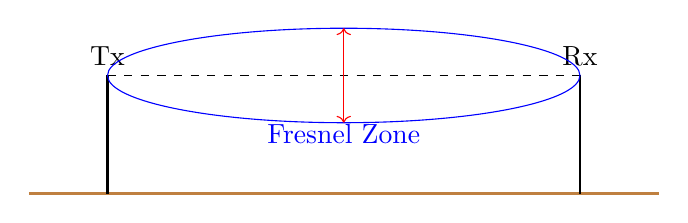
\begin{tikzpicture}
    % Ground
    \draw[thick, brown] (-4,-1) -- (4,-1);
    
    % Antennas
    \draw[thick] (-3,-1) -- (-3,0.5) node[above] {Tx};
    \draw[thick] (3,-1) -- (3,0.5) node[above] {Rx};
    
    % Line of Sight
    \draw[dashed] (-3,0.5) -- (3,0.5);
    
    % Fresnel Zone (Ellipsoid approximation)
    \draw[blue] (0,0.5) ellipse (3cm and 0.6cm);
    \node[blue, below] at (0,0) {Fresnel Zone};
    
    % Obstruction check arrows
    \draw[<->, red] (0, -0.1) -- (0, 1.1);
    
\end{tikzpicture}
\end{center}
\end{purplebox}

\setcounter{chapter}{4}
\setcounter{section}{0}
\chapter*{Appendix D: Gradient operator}
\addcontentsline{toc}{chapter}{Appendix D: Gradient operator}

The gradient of a scalar-valued function $f(x)$ of vector argument $x$, denoted by $\nabla_{x}f(x)$ yields a vector-valued function that, at each point $x$, identifies the direction of greatest increase of $f(\cdot)$, with a magnitude that equals the corresponding rate of increase. It is nothing but the generalization to multiple dimensions of the standard one-dimensional derivative. In rectangular coordinates, where $x=[x_{0}, x_{1}, x_{2}]^T$,
\begin{equation}
    \nabla f(x_{0},x_{1},x_{2})=\frac{\partial f(x_{0},x_{1},x_{2})}{\partial x_{0}}e_{0}+\frac{\partial f(x_{0},x_{1},x_{2})}{\partial x_{1}}e_{1}+\frac{\partial f(x_{0},x_{1},x_{2})}{\partial x_{2}}e_{2}, \tag{D.1}
\end{equation}
where $e_{0}$, $e_{1}$, and $e_{2}$ are unit vectors along the corresponding coordinates. More generally, for vectors with an arbitrary number of dimensions, and with the allowance of them being complex, we can compactly write
\begin{equation}
    [\nabla_{x}f(x)]_{j}=\frac{\partial f(x)}{\partial[x^{*}]_{j}}, \tag{D.2}
\end{equation}
which can be further extended to express the gradient of a scalar-valued function $f(X)$ of a complex matrix argument $X$ as
\begin{equation}
    [\nabla_{X}f(X)]_{i,j}=\frac{\partial f(X)}{\partial[X^{*}]_{i,j}}. \tag{D.3}
\end{equation}

\begin{greenbox}[Example D.1]
For the linear function of complex matrix argument $f(X)=\text{tr}(R_{0}X^{*}R_{1})$,
\begin{equation}
    \nabla_{X}\text{tr}(R_{0}X^{*}R_{1})=R_{1}R_{0} \tag{D.4}
\end{equation}
and, as a corollary
\begin{equation}
    \nabla_{x}(x^{*}r)=r. \tag{D.5}
\end{equation}
Furthermore, because a vector and its conjugate can be regarded as independent for the purpose of gradient computations,
\begin{equation}
    \nabla_{x}(r^{*}x)=0. \tag{D.6}
\end{equation}
\end{greenbox}

\begin{greenbox}[Example D.2]
For the quadratic form $f(x)=x^{*}Rx,$ the gradient equals
\begin{equation}
    \nabla_{x}(x^{*}Rx)=Rx \tag{D.7}
\end{equation}
\end{greenbox}

\begin{greenbox}[Example D.3]
While, for $f(X)=\text{tr}(R_{0}XR_{1}X^{*})$
\begin{equation}
    \nabla_{X}\text{tr}(R_{0}XR_{1}X^{*})=R_{0}XR_{1} \tag{D.8}
\end{equation}
\end{greenbox}

A scalar function of matrix argument that appears often in this text is $f(X)=\log_{e}\det(X),$ with gradient
\begin{equation}
    \nabla_{X}\log_{e}\det(X)=X^{-1}. \tag{D.9}
\end{equation}
From this expression, in turn, (D.8) and the chain rule of differentiation lead to
\begin{equation}
    \nabla_{X}\log_{e}\det(I+X^{*}R_{0}XR_{1})=R_{0}XR_{1}(I+X^{*}R_{0}XR_{1})^{-1}. \tag{D.10}
\end{equation}
For definitions of the gradient operator in cylindrical and spherical coordinates, the reader is referred to specialized literature.

\setcounter{chapter}{5}
\setcounter{section}{0}
\chapter*{Appendix E: Special functions}
\addcontentsline{toc}{chapter}{Appendix E: Special functions}

In order to maximize the generality, elegance, and meaning of their analysis, researchers strive for closed-form results, meaning a combination and composition of elementary functions via the four basic operations. These elementary functions include algebraic functions (solutions of a polynomial equation with integer coefficients) and transcendental functions (including exponentials, logarithms, trigonometric functions, and their inverses).

There are other functions that, while not elementary, appear frequently enough and display sufficiently important properties to have their own names and to be readily tabulated or computable. It is common to relax the interpretation of "closed-form" to also encompass expressions involving these special functions. In this appendix, we survey the special functions that appear throughout this textbook.

\section{Gamma function}
Perhaps the most common special function, and therefore the least special of them all, is the gamma function. For arguments whose real part is positive,
\begin{equation}
    \Gamma(z)=\int_{0}^{\infty}\xi^{z-1}e^{-\xi}d\xi, \tag{E.1}
\end{equation}
which, for positive integers arguments, reduces to $\Gamma(n)=(n-1)!$ indicating that the gamma function can be interpreted as an interpolator for the factorial function. For noninteger arguments, the best known value is $\Gamma(1/2)=\sqrt{\pi}$.

Partial integrals with the same integrand as (E.1) are referred to as incomplete gamma functions, of which two varieties exist: the upper incomplete gamma function
\begin{equation}
    \Gamma(z,s)=\int_{s}^{\infty}\xi^{z-1}e^{-\xi}d\xi, \tag{E.2}
\end{equation}
and the lower incomplete gamma function
\begin{equation}
    \gamma(z,s)=\int_{0}^{s}\xi^{z-1}e^{-\xi}d\xi. \tag{E.3}
\end{equation}

\section{Digamma function}
The digamma function is the logarithmic derivative of the gamma function, i.e.,
\begin{equation}
    \psi(z)=\frac{d}{dz}\log_{e}\Gamma(z) = \frac{\dot{\Gamma}(z)}{\Gamma(z)} \tag{E.4}
\end{equation}
which, for integer arguments, can be expressed as
\begin{equation}
    \psi(N)=-\gamma_{\text{EM}}+\sum_{l=1}^{N-1}\frac{1}{l} \tag{E.5}
\end{equation}
given the Euler-Mascheroni constant
\begin{equation}
    \gamma_{\text{EM}}=\lim_{N\rightarrow\infty}\left(\sum_{n=1}^{N}\frac{1}{n}-\log_{e}N\right) \approx 0.5772 \tag{E.6}
\end{equation}
The digamma function satisfies the recursion
\begin{equation}
    \psi(N+1)=1+\frac{1}{N}\sum_{n=1}^{N}\psi(n). \tag{E.7}
\end{equation}

\section{Exponential integrals}
For real nonzero arguments, the exponential integral function is
\begin{equation}
    \mathcal{E}_{i}(z)=\int_{-\infty}^{z}\frac{e^{\xi}}{\xi}d\xi, \tag{E.10}
\end{equation}
from which a class of functions, parameterized by an order $n$, is defined as
\begin{equation}
    \mathcal{E}_{n}(z)=\int_{1}^{\infty}\frac{e^{-z\xi}}{\xi^{n}}d\xi. \tag{E.11}
\end{equation}
These functions, which we loosely refer to as exponential integrals, are related with the gamma function via
\begin{equation}
    \mathcal{E}_{n}(z)=z^{n-1}\Gamma(1-n,z), \tag{E.12}
\end{equation}
with the most commonly encountered exponential integral being
\begin{equation}
    \mathcal{E}_{1}(z)=-\mathcal{E}_{i}(-z) = \Gamma(0,z). \tag{E.13}
\end{equation}

\section{Bessel functions}
Bessel functions are solutions to a famed differential equation, Bessel's equation. These solutions are parameterized by an order, the most important such orders being integers or half-integers. Bessel functions of the first kind, denoted by $J_{n}(x)$, are solutions that are finite at the origin for integer $n$. They can be expressed as an infinite series or in the integral forms
\begin{equation}
    J_{n}(x)=\frac{1}{2\pi}\int_{-\pi}^{\pi}e^{-j(n\xi-x\sin\xi)}d\xi = \frac{1}{\pi}\int_{0}^{\pi}\cos(n\xi-x\sin\xi)d\xi. \tag{E.15}
\end{equation}
From $J_{n}(\cdot)$, one can further define the modified Bessel functions of the first kind as
\begin{equation}
    I_{n}(x)=j^{-n}J_{n}(jx) \tag{E.17}
\end{equation}
and, in due course, the modified Bessel functions of the second kind as
\begin{equation}
    K_{n}(x)=\frac{\pi}{2}\frac{I_{-n}(x)-I_{n}(x)}{\sin(n\pi)}. \tag{E.18}
\end{equation}

\section{Q-function}
The Q-function is the tail probability of a standard Gaussian distribution. If $x\sim\mathcal{N}(0,1)$, then $Q(x)=\mathbb{P}[x>x]$ and thus the CDF of $x$ satisfies $F_{x}(x)=1-Q(x)$. The usual form for $Q(\cdot)$ is
\begin{equation}
    Q(x)=\frac{1}{\sqrt{2\pi}}\int_{x}^{\infty}e^{-\xi^{2}/2}d\xi, \tag{E.19}
\end{equation}
which can be rewritten as the finite-range integral
\begin{equation}
    Q(x)=\frac{1}{\pi}\int_{0}^{\pi/2}\exp\left(-\frac{x^{2}}{2\sin^{2}\phi}\right)d\phi. \tag{E.20}
\end{equation}
For positive arguments, the Q-function can be bounded as
\begin{equation}
    \frac{x}{1+x^{2}}\frac{e^{-x^{2}/2}}{\sqrt{2\pi}} < Q(x) < \frac{1}{x}\frac{e^{-x^{2}/2}}{\sqrt{2\pi}}, \tag{E.21}
\end{equation}
where the upper bound can be relaxed into the popular Chernoff bound
\begin{equation}
    Q(x)<\frac{1}{2}e^{-x^{2}/2}. \tag{E.22}
\end{equation}
Other upper and lower bounds are available in the literature. Alternatively, a widely valid approximation is
\begin{equation}
    Q(x)\approx\frac{1}{\frac{\pi-1}{\pi}x+\frac{1}{\pi}\sqrt{x^{2}+2\pi}}\frac{e^{-x^{2}/2}}{\sqrt{2\pi}}, \tag{E.23}
\end{equation}
which, like the bounds, evidences that the tail decays exponentially fast. One can also relate the Q-function with the complementary error function via
\begin{equation}
    Q(x)=\frac{1}{2}\text{erfc}\left(\frac{x}{\sqrt{2}}\right), \quad \text{erfc}(x)=\frac{2}{\sqrt{\pi}}\int_{x}^{\infty}e^{-\xi^{2}}d\xi. \tag{E.24}
\end{equation}

\section{Hypergeometric functions}
A hypergeometric function ${}_{p}F_{q}(a_{0},...,a_{p-1};b_{0},...,b_{q-1};x)$ is defined by its series being hypergeometric, meaning that the ratio of consecutive terms is a rational function of the summation index. If $c_{n}$ and $c_{n+1}$ are the $n$th and $(n+1)$th terms in the series, then
\begin{equation}
    \frac{c_{n+1}}{c_{n}}=\frac{P(n)}{Q(n)}, \tag{E.26}
\end{equation}
where $P(n)$ and $Q(n)$ are polynomials. We identify two hypergeometric functions in particular.
\begin{itemize}
    \item The Kummer confluent hypergeometric function is
    \begin{equation}
        {}_{1}F_{1}(a;b;x)=\sum_{n=0}^{\infty}\frac{(a)_{n}}{(b)_{n}}\frac{x^{n}}{n!}. \tag{E.27}
    \end{equation}
    where $(a)_{n}=x\cdot(x+1)\cdot\cdot\cdot(x+n-1)$ with $(a)_{0}=1$. In integral form,
    \begin{equation}
        {}_{1}F_{1}(a;b;x)=\frac{\Gamma(b)}{\Gamma(b-a)\Gamma(a)}\int_{0}^{1}e^{xt}t^{a-1}(1-t)^{b-a-1}dt. \tag{E.28}
    \end{equation}
    \item The Gauss hypergeometric function is
    \begin{equation}
        {}_{2}F_{1}(a_{0},a_{1};b;x)=\sum_{n=0}^{\infty}\frac{(a_{0})_{n}(a_{1})_{n}}{(b)_{n}}\frac{x^{n}}{n!}. \tag{E.29}
    \end{equation}
\end{itemize}

\setcounter{chapter}{6}
\setcounter{section}{0}
\chapter*{Appendix F: Landau symbols}
\addcontentsline{toc}{chapter}{Appendix F: Landau symbols}

The Landau symbols $\mathcal{O}(\cdot)$ and $o(\cdot)$ allow describing, in terms of simpler functions, the limiting behavior of a function as its argument approaches a particular value or tends to infinity. We present these two symbols in the simplest possible way that suffices for their usage in this book.

A function $f(x)$ is said to be $\mathcal{O}(g(x))$, with $g(\cdot)$ being another—ideally simpler—function, if
\begin{equation}
    |f(x)|\le b|g(x)| \tag{F.1}
\end{equation}
for some constant $b$ and all values of $x$.

In turn, $f(x)$ is said to be $o(g(x))$ if
\begin{equation}
    \frac{f(x)}{g(x)}\rightarrow0 \tag{F.2}
\end{equation}
for $x$ approaching a certain value or tending to infinity, depending on the behavior being described.

\setcounter{chapter}{7}
\setcounter{section}{0}
\chapter*{Appendix G: Convex optimization}
\addcontentsline{toc}{chapter}{Appendix G: Convex optimization}

\section{Convex sets}
A set is convex if it contains all segments between any two of its points, meaning that it is free of indentations. An example of convex set is the one depicted in Fig. 5.4.

\section{Convex and concave functions}
A real-valued function $f(x)$ is convex if it satisfies
\begin{equation}
    f(\theta x_{0}+(1-\theta)x_{1})\le\theta f(x_{0})+(1-\theta)f(x_{1}) \tag{G.1}
\end{equation}
for any real vectors $x_{0}$ and $x_{1}$ on a certain domain and for every real scalar $\theta\in[0,1]$. This implies that the graph of the function lies below any chord, i.e., below any segment connecting two points of that graph. If the inequality in (G.1) is strict, then the function is strictly convex. Conversely, if the inequality is a strict equality, then the function is linear.

A function $f(\cdot)$ is concave (respectively strictly concave) if $-f(\cdot)$ is convex (respectively strictly convex), meaning that its graph lies above any chord. Examples of concave functions are shown in Fig. G.1.

\begin{center}
\begin{tikzpicture}
    % First plot (Nonmonotonic concave)
    \begin{scope}
        \draw[<->] (0,2) node[left] {$f(x)$} -- (0,0) -- (3,0) node[below] {$x$};
        \draw[thick] (0.2,0.8) .. controls (1,2.2) and (2,2.2) .. (2.8,1.2);
    \end{scope}

    % Second plot (Monotonically increasing concave)
    \begin{scope}[xshift=5cm]
        \draw[<->] (0,2) node[left] {$f(x)$} -- (0,0) -- (3,0) node[below] {$x$};
        \draw[thick] (0.2,0.5) .. controls (1,1.5) and (2,1.8) .. (2.8,2.0);
    \end{scope}
\end{tikzpicture}
\captionof{figure}{Fig G.1: Left, nonmonotonic concave function of a real scalar argument. Right, monotonically increasing concave function.}
\end{center}

If $f(\cdot)$ is concave, then the problem of finding its maximum over a convex set readily maps to (G.2) with the objective function given by $-f(\cdot)$.

\section{Convex optimization problems}
An optimization problem has the form
\begin{align}
    \text{minimize } & f(x) \nonumber \\
    \text{subject to } & g_{i}(x)\le d_{i} \quad i=0,...,N-1 \tag{G.2}
\end{align}
where $f(\cdot)$ is the objective or cost function whereas $g_{i}(\cdot)$ are the constraint functions. The solution $x^{*}$ satisfies $f(x^{*})\le f(x)$ for every vector $x$ meeting the $N$ constraints.

If $f(\cdot)$ as well as $g_{0}(\cdot),...,g_{N-1}(\cdot)$ are convex, then the optimization problem is said to be convex. This means that the set defined by the constraint functions, over which the optimum is to be found, is convex and the objective function thereon is also convex. Convex problems can be interpreted as a generalization of linear problems, which are those where $f(\cdot)$ and $g_{0}(\cdot),...,g_{N-1}(\cdot)$ are linear functions.

While, in general, the solution of generic optimizations may pose considerable difficulty, convex problems can be solved reliably and efficiently even when they involve vectors with many dimensions. For an overview of convex optimization procedures and algorithms, the reader is referred to specialized textbooks. Convex optimization problems arise frequently in communications and, in particular, in MIMO.

A key advantage of convex problems over nonconvex ones is that, if a local minimum exists, then it is a global minimum. As a result, any set of necessary conditions characterizing a minimum are also sufficient for global optimality.

\section{KKT optimality conditions}
The Karush-Kuhn-Tucker (KKT) conditions are necessary and sufficient conditions characterizing the solution to a convex problem. In order to present them, it is useful to rewrite (G.2) distinguishing between those constraints that are inequalities and those that are strict equalities. Also, by suitably modifying the constraint functions, we can set all the constraints to zero, obtaining
\begin{align}
    \text{min } & f(x) \nonumber \\
    \text{s.t. } & g_{i}(x)\le0 \quad i=0,...,M^{\prime}-1 \tag{G.3} \\
    & h_{j}(x)=0 \quad j=0,...,M-1 \nonumber
\end{align}

Then, the KKT conditions characterizing $x^*$ are
\begin{align}
    \nabla f(x^{*})+\sum_{i=0}^{M^{\prime}-1}\lambda_{i}^{\prime}\nabla g_{i}(x^{*})+\sum_{j=0}^{M-1}\lambda_{j}\nabla h_{j}(x^{*})=0 \tag{G.4} \\
    g_{i}(x^{*})\le0 \quad i=0,...,M^{\prime}-1 \nonumber \\
    h_{j}(x^{*})=0 \quad j=0,...,M-1 \nonumber \\
    \lambda_{i}^{\prime}\ge0 \quad i=0,...,M^{\prime}-1 \nonumber \\
    \lambda_{i}^{\prime}g_{i}(x^{*})=0 \quad i=0,...,M^{\prime}-1 \nonumber
\end{align}
where $\lambda_{0}^{\prime},...,\lambda_{M^{\prime}-1}^{\prime}$ and $\lambda_{0},...,\lambda_{M-1}$ are the so-called KKT multipliers.

The KKT conditions play an important role in convex optimization, often serving as targets for the algorithms. Moreover, sometimes the KKT conditions can be analytically resolved, yielding expressions that characterize the solution directly.

\begin{purplebox}[Note]
\textbf{da sapere} (to know)
\end{purplebox}

\section{Lagrange multipliers}
If there are no inequality constraints, but only equality ones, the solution of the KKT conditions reverts to the method of Lagrange multipliers. Consider the problem
\begin{align}
    \text{min } & f(x) \nonumber \\
    \text{s.t. } & h_{j}(x)=0 \quad j=0,...,M-1 \tag{G.5}
\end{align}
If we augment the objective function with a weighted sum of the constraint functions we obtain the so-called Lagrangian function
\begin{equation}
    L(x,\lambda_{0},...,\lambda_{M-1})=f(x)+\sum_{j=0}^{M-1}\lambda_{j}h_{j}(x), \tag{G.6}
\end{equation}
where $\lambda_{0},...,\lambda_{M-1}$ are termed Lagrange multipliers.

Any point $x^{*}$ where all partial derivatives of $L(\cdot)$ are zero corresponds to an extreme point (minimum or maximum) that satisfies the equality constraints. If $f(\cdot)$ is convex or concave, then this extreme point is guaranteed to be the global one. The conditions satisfied by $x^{*}$ can be written as
\begin{align}
    \nabla_{x}L(x^{*})=\nabla f(x^{*})+\sum_{j=0}^{M-1}\lambda_{j}\nabla h_{j}(x^{*})=0 \tag{G.7} \\
    h_{j}(x^{*})=0 \quad j=0,...,M-1 \nonumber
\end{align}
which, indeed, can be seen to be a special case of (G.4).

Often, the objective functions encountered in communications are not only convex or concave, but further monotonic in quantities of interest (see Fig. G.1). Taking advantage of that, inequality constraints can be tightened into strict equalities, paving the way for the application of Lagrange multipliers directly, rather than the more general KKT conditions. Examples include the spectral efficiency or the error probability, both of which improve monotonically with the signal power in most settings; then, any applicable power constraints can be considered directly as equalities.

\section{Jensen's inequality}
As stated earlier, the inequality in (G.1) reflects that the graph of a convex function lies below any chord. This generalizes into the widely utilized Jensen's inequality. Given a convex function $f(x)$ and the vectors $x_{0},...,x_{N-1}$ in its domain,
\begin{equation}
    f\left(\frac{\sum_{i=0}^{N-1}a_{i}x_{i}}{\sum_{i=0}^{N-1}a_{i}}\right)\le\frac{\sum_{i=0}^{N-1}a_{i}f(x_{i})}{\sum_{i=0}^{N-1}a_{i}} \tag{G.8}
\end{equation}
for any positive coefficients $a_{0},...,a_{N-1}$. As a special case, if $a_{i}=1$ for $i=0,...,N-1$, the weighted sum gives the average and thus, if the vectors are random variables, we can write
\begin{equation}
    f(\mathbb{E}[x])\le\mathbb{E}[f(x)]. \tag{G.9}
\end{equation}
If $f(\cdot)$ is concave, rather than convex, the above inequalities are simply reversed.

\end{document}